\chapter{Strumenti fondamentali} \label{tools}
Prima di addentrarci nella trattazione del teorema, richiamiamo alcune nozioni alla base di quanto diremo più avanti. 
In particolare, avere chiare queste informazioni risulterà cruciale per assicurarsi di aver compreso a fondo il significato delle ipotesi che richiederemo e le tecniche dimostrative utilizzate.

Prima di tutto, anche per cominciare a prendere familiarità con la notazione, ripassiamo la nomenclatura delle equazioni equazioni differenziali di ordine $k$, e di conseguenza degli operatori ad esse associate, con una tabella riassuntiva:
\begin{center}
\renewcommand{\arraystretch}{2}
\begin{tabular}{l l} 
\hline \hline
 Lineare & $\sum_{|\alpha |\leq k} a_\alpha \, D^\alpha u = f$ \\
 \hline
 \vspace{-2mm}
 Quasi-lineare & $\sum_{|\alpha |= k} a_\alpha (x,D^\beta u) \, D^\alpha u +  a_0(x,D^\beta u)= f,$\\
 & $\quad |\beta |<k $ \\
 \hline
 Non lineare & $F(x,D^\alpha u)=0, \quad |\alpha | \leq k$ \\
 \hline
 In forma normale & $D_{t}^k u = G(x,t, D^\alpha_x D^j_t u), \quad |\alpha |+j \leq k, \, j < k$ \\
 \hline \hline
\end{tabular}
\end{center}
\begin{remark}
Nel caso di equazione in forma normale si dividono le variabili tra spazio $x\in \mathbb{R}^{n-1}$ e tempo $t$, per una ragione che sarà chiara una volta conclusa la lettura di questo capitolo.
\end{remark}
Cominciamo già ad anticipare che, successivamente, i coefficienti e le funzioni che definiscono le equazioni li assumeremo molto regolari, per la precisione analitici (ovvero localmente sviluppabili in serie di potenze).\\
Alla luce di quanto detto fin'ora, ci rendiamo conto di come ci sarebbero già alcuni aspetti su cui sarebbe importante soffermarsi.
Ma per essere più ordinati riassumiamo le nostre tematiche di interesse in quattro punti, i quali rispecchiano la struttura dei questo capitolo:
\begin{enumerate}
\item \textbf{superfici caratteristiche}: ovvero quelle superfici in $\mathbb{R}^n$ che sono strettamente legate alla forma dell'equazione in osservazione e che possono essere fonte di problemi quando si decide di assegnare dei dati Cauchy su di esse;
\item \textbf{metodo delle caratteristiche}: nel caso di equazioni, anche non lineari, del primo ordine è possibile vedere un'EDP come un sistema di EDO dipendente da un parametro;
\item \textbf{problemi di Cauchy}: l'unica tipologia di problemi di cui ci occuperemo;
\item \textbf{serie di potenze}: costituiscono le fondamenta del concetto di funzione analitica (e olomorfa nel caso dei numeri complessi), ovvero l'unica tipologia di funzioni che cercheremo come soluzione. 
\end{enumerate}

\newpage
\section{Superfici caratteristiche}
Superfici caratteristiche per op. lineari
$L$ operatore differenziale lineare.
\begin{definition}
Forma caratteristica di $L$:\\ $\chi_L(x,\xi)=\sum\limits_{|\alpha |= k} a_\alpha(x) \, \xi^\alpha \quad \text{con} \quad x,\xi \in \mathbb{R}^n$
\end{definition}

\begin{definition}
Varietà caratteristica di $L$ in $x$:\\ $\text{char}_x (L)= \{ \xi \neq 0 : \chi_L(x,\xi)=0 \}$
\end{definition}



\begin{definition}
$\Gamma$ superficie caratteristica per $L$ in $x \iff \nu(x) \in\text{char}_x (L)$
\end{definition}

\begin{remark}
Caso di operatore del $1$° ordine: $A=(a_1,\ldots ,a_n)$ tangente a $\Gamma$.\\
Utile per generalizzazioni successive.
\end{remark}

Significato
$$\xi \in \text{char}_x (L)$$
in $x$ $L$ non è ``propriamente'' di ordine $k$ nella direzione $\xi$.
\vspace{5mm}
$$\Gamma \text{ non caratteristica }$$ 
date su $\Gamma$ $D^i_\nu u \,(i<k)$ di una soluzione $u$
è possibile calcolare tutte le sue derivate parziali su $\Gamma$.


Op. quasi-lineari $1$° ordine

\begin{itemize}
\item $\gamma (s): \mathbb{R}^{n-1}\rightarrow \mathbb{R}^n$ parametrizzazione locale di $\Gamma$
\item $u = \phi$ su $\Gamma$ dato di Cauchy
\end{itemize}

\begin{definition}
$\Gamma$ non caratteristica in $x_0=\gamma (s_0)$\\
\begin{equation*}
\iff \det
\underbrace{
\left[
\begin{matrix}
D_{s_1}\gamma_1 & \cdots & D_{s_{n-1}}\gamma_1 \\
\vdots &  & \vdots \\
D_{s_1}\gamma_n & \cdots & D_{s_{n-1}}\gamma_n \\
\end{matrix}\;\right|}_{\text{span del piano tangente}} \,
\left.
\begin{matrix}
a_1(\gamma, \phi(\gamma))\\
\vdots\\
a_n(\gamma, \phi(\gamma))\\
\end{matrix}\right] (s_0) \neq 0
\end{equation*}
\end{definition}

\newpage
\section{Metodo delle caratteristiche}
I problemi seguenti sono \textbf{equivalenti}.
\begin{equation} \label{edpquasilin}
\text{EDP : }
\begin{cases}
\sum a_j(x,u)D_{x_j} u = b(x,u)\\
u = \phi \text{ su } \Gamma
\end{cases} 
\end{equation}
\begin{equation}
\text{EDO : }
\begin{cases}
D_t \, x = A(x,y) \; \footnotemark \\
D_t \, y = b(x,y)\\ 
x(0)=x_0\\ 
y(0) = \phi (x_0) \quad \forall x_0 \in \Gamma
\end{cases} 
\end{equation}
Dove $y = u(x)$ e $A(x,y)=[a_1(x,y),\ldots ,a_n(x,y)]$.
\footnotetext{le soluzioni $x$ vengono dette \textit{curve caratteristiche}}


\begin{theorem}
\hpth{
\text{Problema \eqref{edpquasilin} } \\
a_j, \, b, \, \phi , \, \Gamma \in C^1\\
\Gamma \text{ non caratteristica}
}{
\exists ! \text{ soluzione } C^1 \text{ in un intorno di } \Gamma
}
\end{theorem}
\begin{proof}
sfruttando il teorema di esistenza e unicità locale per EDO
\end{proof}

si può generalizzare tutto (superfici caratteristiche e metodo delle caratteristiche) al caso non lineare (primo ordine), non lo facciamo perché il metodo delle caratteristiche ci servirà solo nel caso quasi lineare e per la def di non caratteristicità seguiamo un altro approccio più rapido ed equivalente.

\newpage
\section{Problemi di Cauchy}
\begin{itemize}
\item Spesso utilizzato quando la superficie dei dati \textbf{non} è un bordo.
\item Necessita anche le \textbf{derivate normali} ($D^j_\nu u$) della soluzione sulla superficie per determinarla univocamente.
\item Porta con sé il rischio di essere \textbf{sovradeterminato} (buono per l'unicità e meno per l'esistenza della soluzione).
\end{itemize}

Non ci preoccupiamo della regolarità delle funzioni perché poi le assumeremo analitiche.
Problema generale
\begin{equation*}
\begin{cases}
F^*(x,D^\alpha u^*)=0 & |\alpha | \leq k, \, F^* \text{ almeno } C^1\\
D^j_\nu u^* = \phi_j^* & \text{su } \Gamma^* \text{ per }j<k 
\end{cases}
\end{equation*}



Mappatura in $t=0$

Detta $\gamma^*$ la parametrizz. locale di $\Gamma^*$, applichiamo la mappa:
$$\Phi (x) = 
\begin{bmatrix}[ccc|c]
x_1 & \cdots & x_{n-1} & x_n-\gamma^* (x_1,\ldots , x_{n-1})
\end{bmatrix}$$
\begin{figure}[H]
\centering
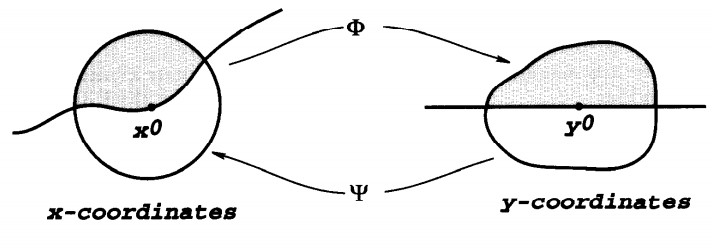
\includegraphics[scale=.5]{flatb}
\caption{Immagine da \cite[cap.8]{Evans}}
\end{figure}



\begin{enumerate}
\item Selezioniamo una variabile privilegiata e chiamiamola ``tempo'':
\begin{align*}
t & \leftarrow x_n \\
x & \leftarrow (x_1,\ldots , x_{n-1})
\end{align*}
\item Chiamiamo $\Gamma_0 = \{t=0\}$.
\item Indichiamo le derivate nel modo seguente: $D^\alpha_x D^j_t u$.
\item Otteniamo il problema ($u^*=u(\Phi)$):
\begin{equation*}
\begin{cases}
F(x,t, D^\alpha_x D^j_t u)=0 & |\alpha | +j \leq k\\
D^j_t u (x,0)= \phi_j(x) & \text{per }j<k 
\end{cases}
\end{equation*}
\end{enumerate}



Superfici non caratteristiche in generale

\begin{definition}
$\Gamma^*$ (o $\Gamma_0$) è non caratteristica $\iff$ l'equazione su $\Gamma_0$ può essere riscritta in \textbf{forma normale} rispetto a $t$.
\end{definition}

\begin{remark}
Si dimostra che è coerente con le definizioni precedenti.
\end{remark}

\begin{remark}
\begin{itemize}
\item Caso lineare $\rightarrow$ condizione sui coefficienti.
\item Caso non lineare $\rightarrow$ validità ipotesi teorema del Dini su $F$.
\end{itemize}
\end{remark}


\newpage
\section{Serie di potenze}
Dando per nota la teoria delle funzioni olomorfe, e di conseguenza anche la teoria base delle funzioni analitiche (reali), in questo paragrafo vogliamo scoprire, o conoscere meglio, solamente degli strumenti molto specifici che ci permetteranno di dimostrare il TCK.

Cominciando dallo studiare uno sviluppo in serie di potenze di una funzione di cui non dobbiamo dimenticarci.
\begin{definition}
Funzione maggiorante: $$\mathcal{M}_{Cr}(x)=\frac{Cr}{r-(x_1+\ldots +x_n)}$$
\end{definition}
Utilizzando il teorema multinomiale, dimostriamo che la questa funzione può essere sviluppata in serie di potenze per $|x|<r/n$, ricavandone l'espressione dei coefficienti $c_\alpha$:
\begin{align*}
\mathcal{M}_{Cr}(x) &= \frac{Cr}{r-(x_1+\ldots +x_n)} = C \sum\limits_{j=0}^\infty \left(\frac{x_1+\ldots +x_n}{r}\right)^j  \\
&= C \sum\limits_{j=0}^\infty \frac{1}{r^j} \sum\limits_\alpha \left( \frac{|\alpha |!}{\alpha !}\right)x^\alpha = \sum\limits_\alpha 
\underbrace{\frac{C|\alpha |!}{\alpha ! \, r^{|\alpha |}}}_{c_\alpha} \, x^\alpha
\end{align*}
$$.$$



Metodo dei maggioranti
\begin{theorem}[utilità del maggiorante]
\begin{equation*}
\begin{cases}
g_\alpha \geq |f_\alpha|\\
\sum g_\alpha x^\alpha \text{ ha raggio di conv. } R
\end{cases}
\implies 
\begin{array}{c}
\sum f_\alpha x^\alpha \\
\text{ha raggio almeno } R
\end{array}
\end{equation*}
\end{theorem}
In questo caso si scrive:  $\sum g_\alpha x^\alpha \gg \sum f_\alpha x^\alpha$.



\begin{theorem}[costruzione del maggiorante]
$\sum f_\alpha x^\alpha$ ha raggio $R \implies \exists \, r<R, \, C>0$ tali che 
$$|f_\alpha | \leq C \frac{1}{r^{|\alpha |}} \leq C \frac{|\alpha |!}{\alpha ! \, r^{|\alpha |}}$$
\end{theorem}



\newpage
\section{Note}
Cosa si intende per superficie analitica\\
superfici caratteristiche e calcolo di tutte le derivate parziali:
\begin{itemize}
\item caso $t=0$
\item caso generale 
\end{itemize}

